% sec_direction.tex
\section{Условие направленности потока (порог устойчивости)}

Следующее условие существования ЭВ связано с его «вихревой» сущностью в виде \textbf{спиралевидных траекторий} движения составляющих его Амеров. Известно, что движение по криволинейным траекториям невозможно без внешнего воздействия, изменяющего направление движения тела или частицы. В представляемой модели единственным внешним воздействием на частицы ЭВ являются соударения с Амерами СЭ, происходящие в условиях кинетического равновесия и отсутствия взаимопроникновения частиц на границе раздела, которые обеспечивают сохранение условий существования \textbf{направленного} движения частиц эфира в вихре. Очевидно, что наличие таких условий указывает на существование кинетической, пространственной и геометрической обусловленности параметров частиц СЭ и ЭВ, которая указывает на направления поиска и варианты подходящих модельных решений.

Следует особо отметить, что СЭ никак не обусловлен существованием или отсутствием ЭВ и организованных форм их объединений в виде материальных тел и систем; иначе говоря, хаотическая форма движения частиц эфира абсолютна и субъектна. Для ЭВ и их объединений, напротив, СЭ, или физический вакуум, является необходимым условием существования, что указывает на субъектность СЭ и его роль главного актора в процессах мироздания и, напротив, объектность материальных тел, включая ЭВ. Вопрос субъектности СЭ и объектности ЭВ на самом деле гораздо шире и глубже обозначенного необходимого условия существования материальных тел и будет раскрываться по мере необходимости при изложении причинно-следственных последовательностей возникновения взаимодействий между ними. Бесконечная вариативность параметров эфирных сред в условиях ничем не ограниченных диапазонов их значений, с одной стороны, и необходимость существования детерминантных ограничений для взаимообусловленности поведения акторов процесса заставляет искать «подсказки» в виде логически и причинно обоснованных аргументов, основанных на особенностях взаимодействия частиц, составляющих эти среды, и позволяющих сузить круг возможных достоверных модельных решений.

Предположение о направленном движении частиц в ЭВ подразумевает, что это движение будет продолжаться в течение всего его жизненного цикла. Замкнутость эфирокинетической системы, равенство потоков импульса через поверхность границы и реактивный характер соударения Амеров допускает такое развитие событий; однако встаёт вопрос о том, что является условием сохранения \textbf{направленности движения} как сущности. Какие должны быть соблюдены условия, чтобы процесс направленного движения Амеров ЭВ, сопровождающийся соударениями между собой в потоке и с Амерами СЭ на границе, не превратился с течением времени в хаотическое движение? Представим себе движущийся в каком-либо направлении поток частиц эфира. Одновременное направленное перемещение всех частиц не ставит под сомнение факта неизменности их концентрации \(n_{\text{эв}}\) в каждый момент времени по всему континууму потока, а также того, что частицы, сталкиваясь, могут увеличивать и уменьшать скорость в попутном направлении, а также обмениваться компонентами скорости с соседними частицами в поперечном основному движению направлениях. По сути, можно с уверенностью предположить, что каждый Амер, движущийся в \textbf{вихревом} потоке, одновременно участвует в двух видах движения, а именно: \textbf{направленном} и \textbf{хаотическом}.

\begin{figure}[h]
\centering
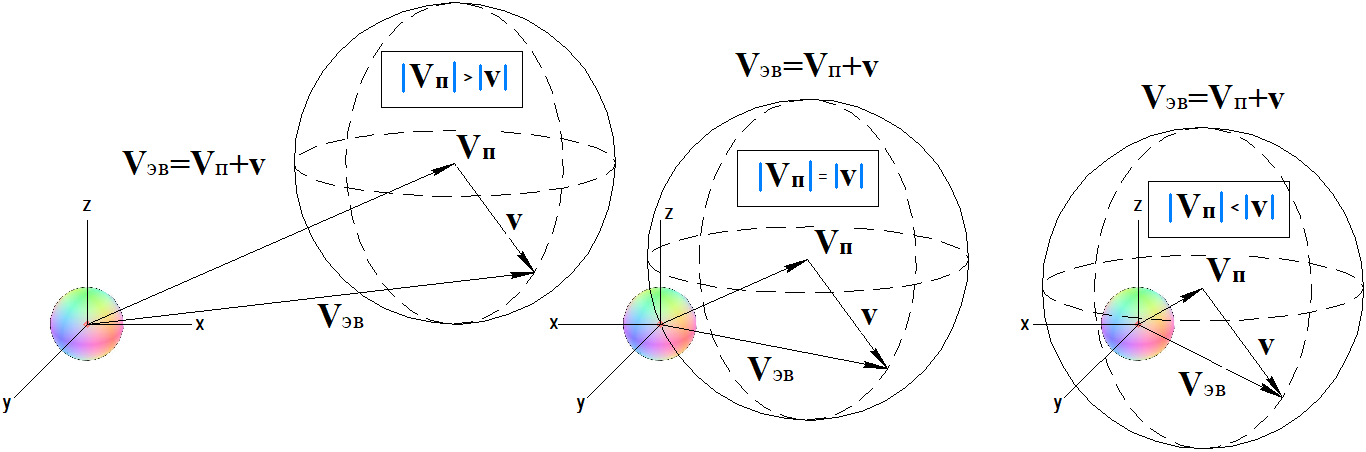
\includegraphics[width=0.9\textwidth]{images/a16.png}
\caption{Диаграммы скоростей Амера в вихревом потоке.}
\label{fig:diagrams}
\end{figure}

Как видно из приведённых рисунков \ref{fig:diagrams}, скорость каждого Амера \(\mathbf{v}_{\text{эв}}\), направленно движущегося в теле ЭВ, представляет собой геометрическую сумму вектора скорости потока \(\mathbf{v}_n\), которой обладает каждый Амер, и текущего вектора скорости хаотического движения \(\mathbf{v}\): \(\mathbf{v}_{\text{эв}} = \mathbf{v}_n + \mathbf{v}\). Эту геометрическую сумму в дальнейшем будем называть \textbf{вихревой скоростью}. Область изменения направлений движения вектора скорости хаотического движения составляет телесный угол внутри сферы, равный \(4\pi\). Направление вектора потока в случае его прямолинейности неизменно, но для движущихся частиц в теле эфирного вихря вектор скорости потока постоянно изменяет направление под внешним воздействием в виде соударений Амеров Свободного эфира на границе вихря. Внешне это очень похоже на кинематическую задачу о равноускоренном движении тела по окружности и, по сути, им является. Однако сейчас стоит другая цель, обозначенная выше.

На рисунках \ref{fig:diagrams} изображены диаграммы скоростей Амеров ЭВ в абсолютной системе отсчёта при различных соотношениях величин скорости потока частиц \(\|\mathbf{v}_n\|\) и среднего значения модуля скорости их хаотического движения \(\|\mathbf{v}\|\). В порядке небольшого отступления: составление различных диаграмм или совершение иных подобных действий не означает «придумывания» каких-либо необходимых «пазлов» модели эфира; автор рассматривает логически возможные физические варианты развития событий, строго следуя избранным инвариантам, и выбирает наиболее вероятные, а значит, удовлетворяющие требованиям детерминантных ограничений в виде «естественного отбора» способных к долговременному существованию вихревых вещественных эфирных структур.

Продолжая, следует отметить, что конец вектора \(\mathbf{v}_{\text{эв}}\) всегда расположен на шаровой поверхности, описываемой вектором хаотической составляющей \(\mathbf{v}\). В случае \(\|\mathbf{v}_n\| = \|\mathbf{v}\|\) (рис. \ref{fig:diagrams}) область изменения направления движения Амеров составляет телесный угол величиной \(2\pi\) и, при этом, существует возможность остановки частиц эфира \(\mathbf{v}_n = -\mathbf{v}\) в абсолютной системе отсчёта, что противоречит избранной нами концепции о движущейся материи, представленной в нашей модели Амерами. Если \(\|\mathbf{v}_n\| < \|\mathbf{v}\|\), то Амер имеет направления для движения внутри телесного угла \(4\pi\), что означает возможность существования обратных потоков частиц эфира, которые, взаимодействуя с основным, трансформируют направленный вид движения Амеров в хаотический, следствием чего будет разрушение эфирного вихря. Таким образом, наилучшим соответствием критерию «направленности» движения частицы отвечает случай \(\|\mathbf{v}_n\| > \|\mathbf{v}\|\). Как итог, на рис. \ref{fig:cone} представлен вектор вихревой скорости Амера \(\mathbf{v}_{\text{эв}}\), прецессирующий внутри конуса с телесным углом \(\Omega\), «скользящий» своим концом по сферической поверхности радиусом \(\|\mathbf{v}\|\).

\begin{figure}[h]
\centering
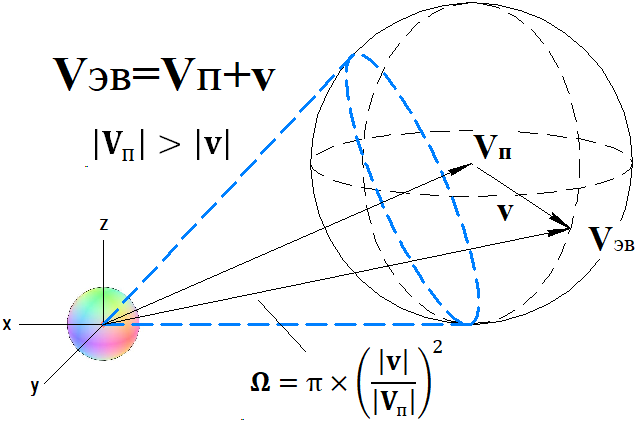
\includegraphics[width=0.45\textwidth]{images/a18.png}
\caption{Телесный угол прецессии вихревой скорости.}
\label{fig:cone}
\end{figure}

Изображённая на рис. \ref{fig:cone} диаграмма скоростей движущегося в вихревом потоке Амера справедлива для усреднённого значения модуля «хаотической» составляющей \(\|\mathbf{v}\|\) его вихревой скорости \(\mathbf{v}_{\text{эв}}\). В действительности длина вектора \(\mathbf{v}\) может отличаться от своего среднего значения в большую или меньшую сторону, что, впрочем, не меняет ситуацию принципиально. Эфирокинетическая структура материи представляемой модели предполагает взаимообусловленность параметров составляющих её частей, находящуюся в строго определённых интервалах их соотношений в пределах допустимых изменений величин, что, по сути, является необходимым детерминантным условием существования материальных тел всех иерархических уровней организации. Иначе говоря, предметом поиска являются не конкретные значения величин параметров систем, а их взаимосвязанные интервалы значений, в пределах которых системы могут существовать в стационарных равновесных состояниях, например, в виде протонов или электронов.

\begin{figure}[h]
\centering
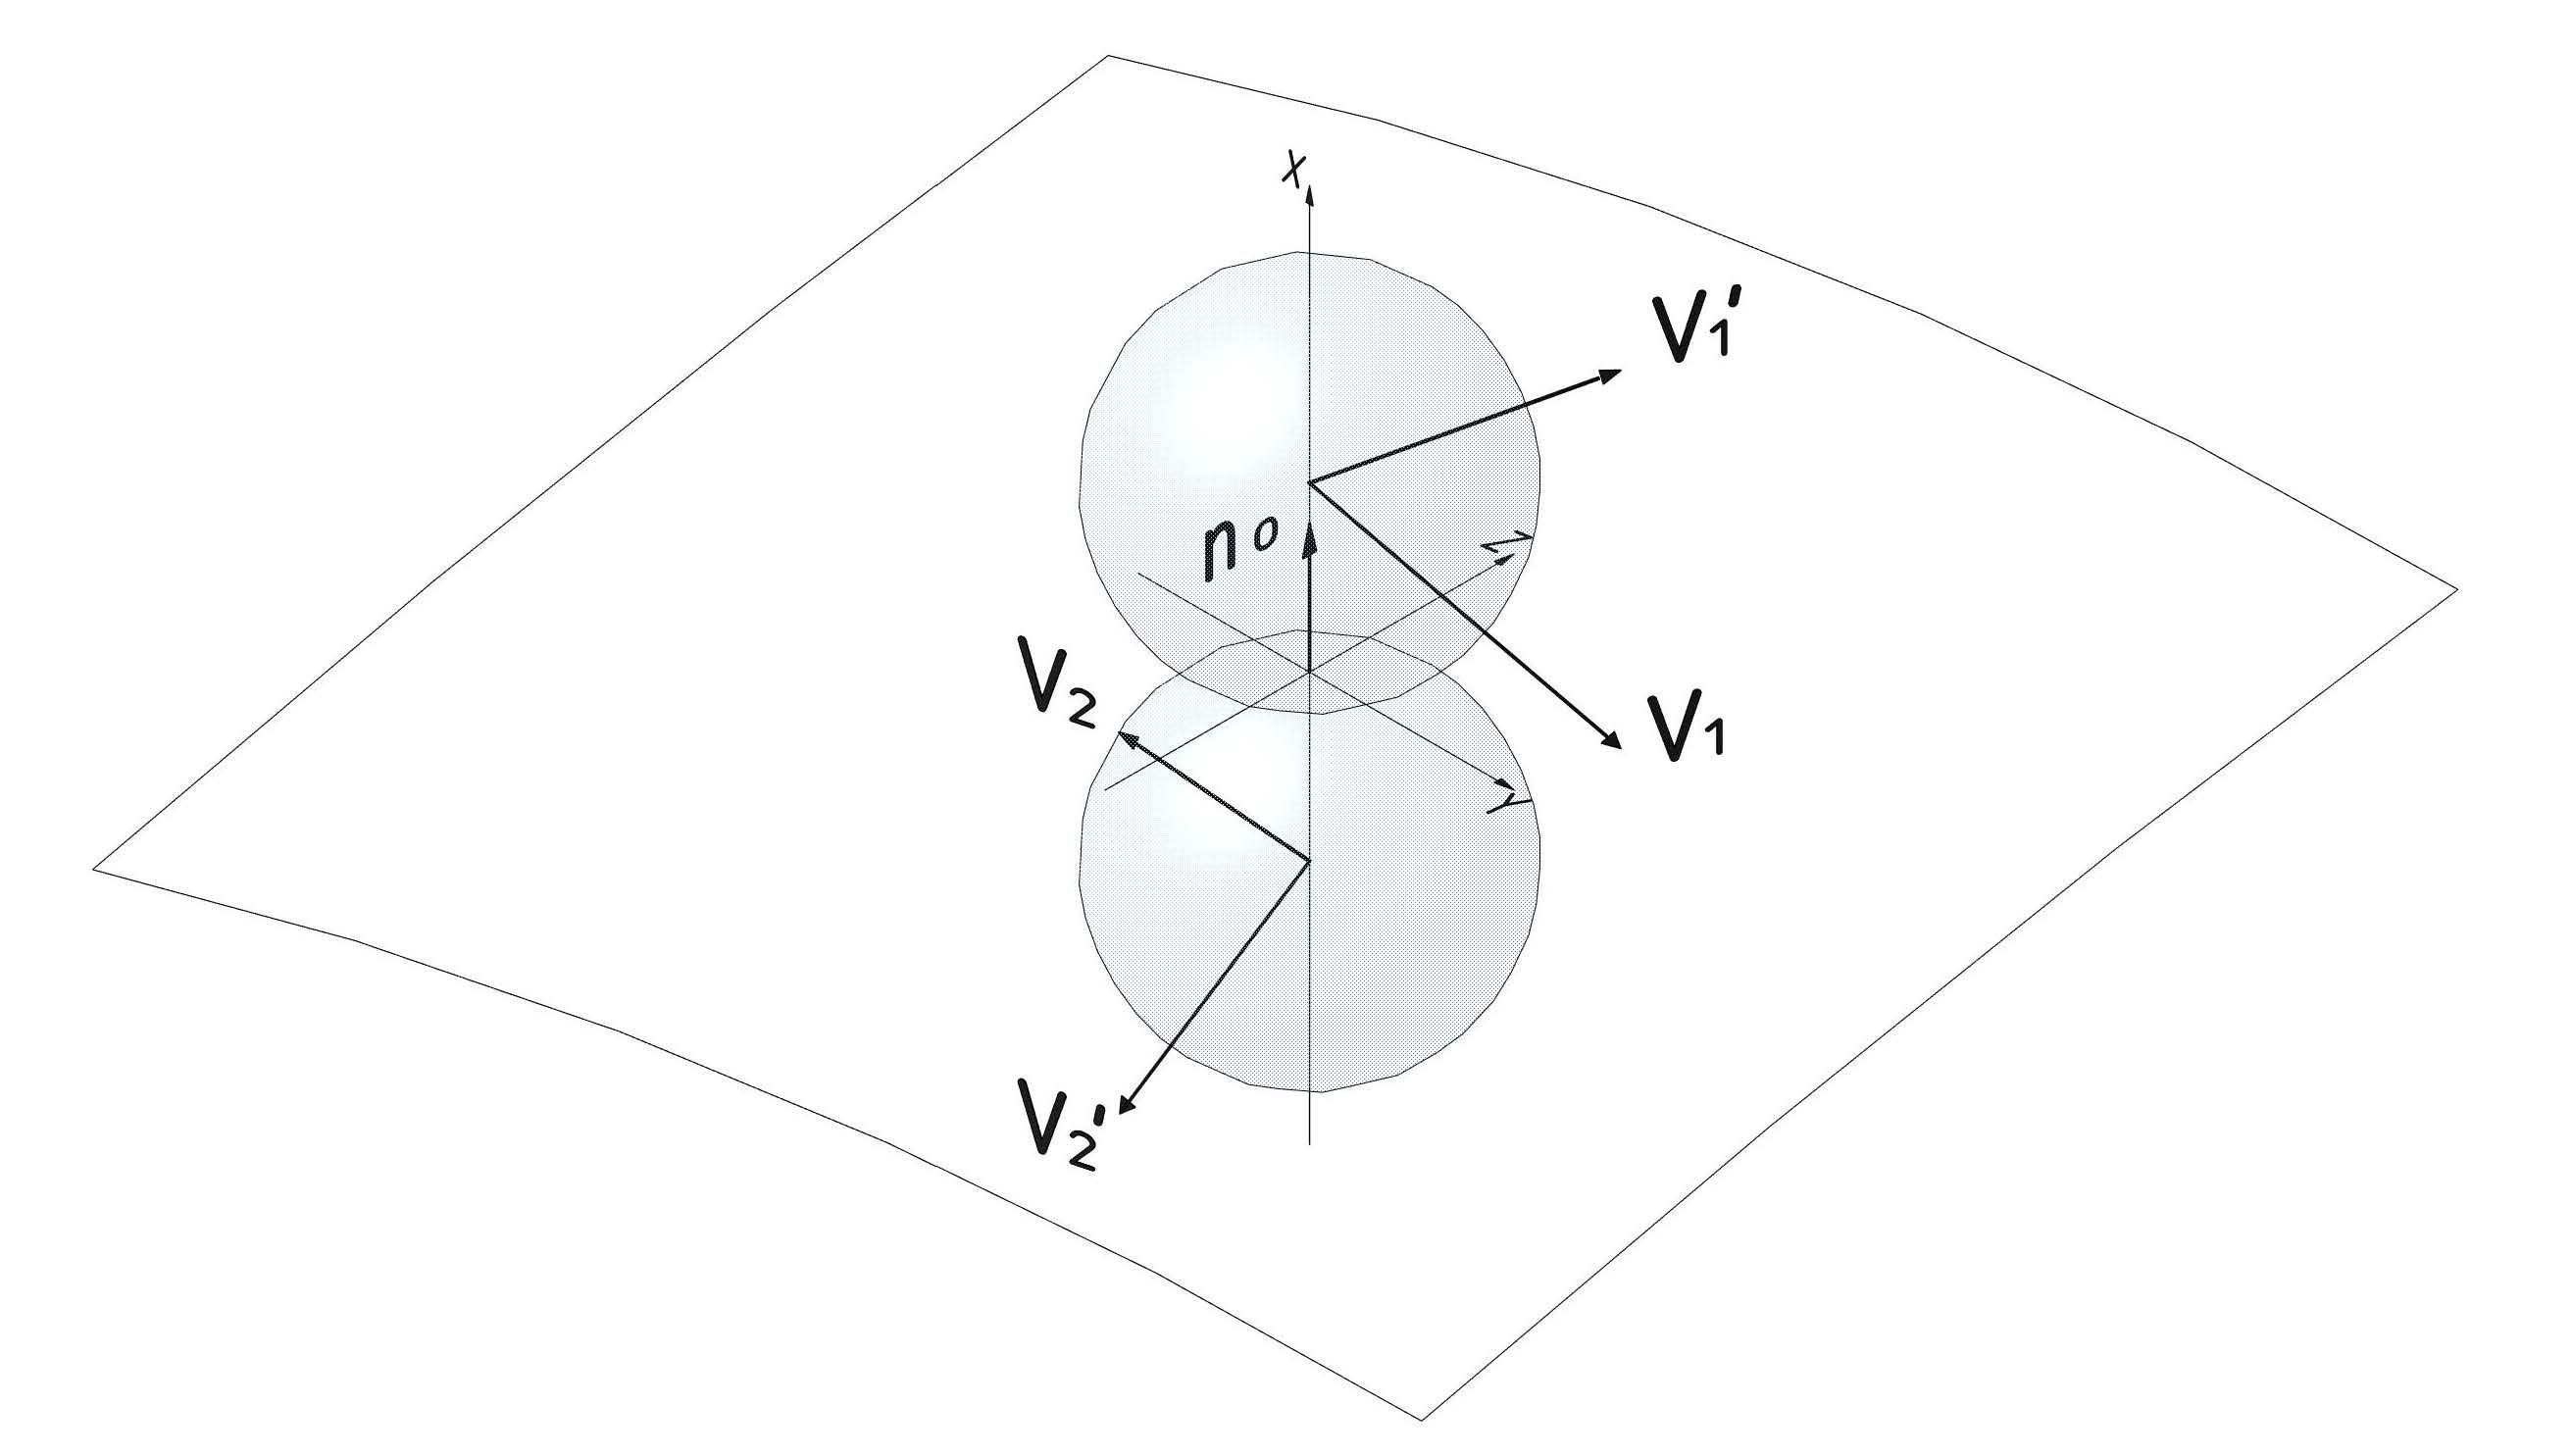
\includegraphics[width=0.55\textwidth]{images/a7.png}
\caption{Соударение на границе.}
\label{fig:boundary_collision}
\end{figure}

Рассмотрим акт соударения двух Амеров (рис. \ref{fig:boundary_collision}) на условной граничной поверхности раздела ЭВ и СЭ. Принимая в учёт изображённую кривизну поверхности, примем верхний Амер за принадлежащий СЭ, а нижний — соответственно, представляющий ЭВ.

\begin{figure}[h]
\centering
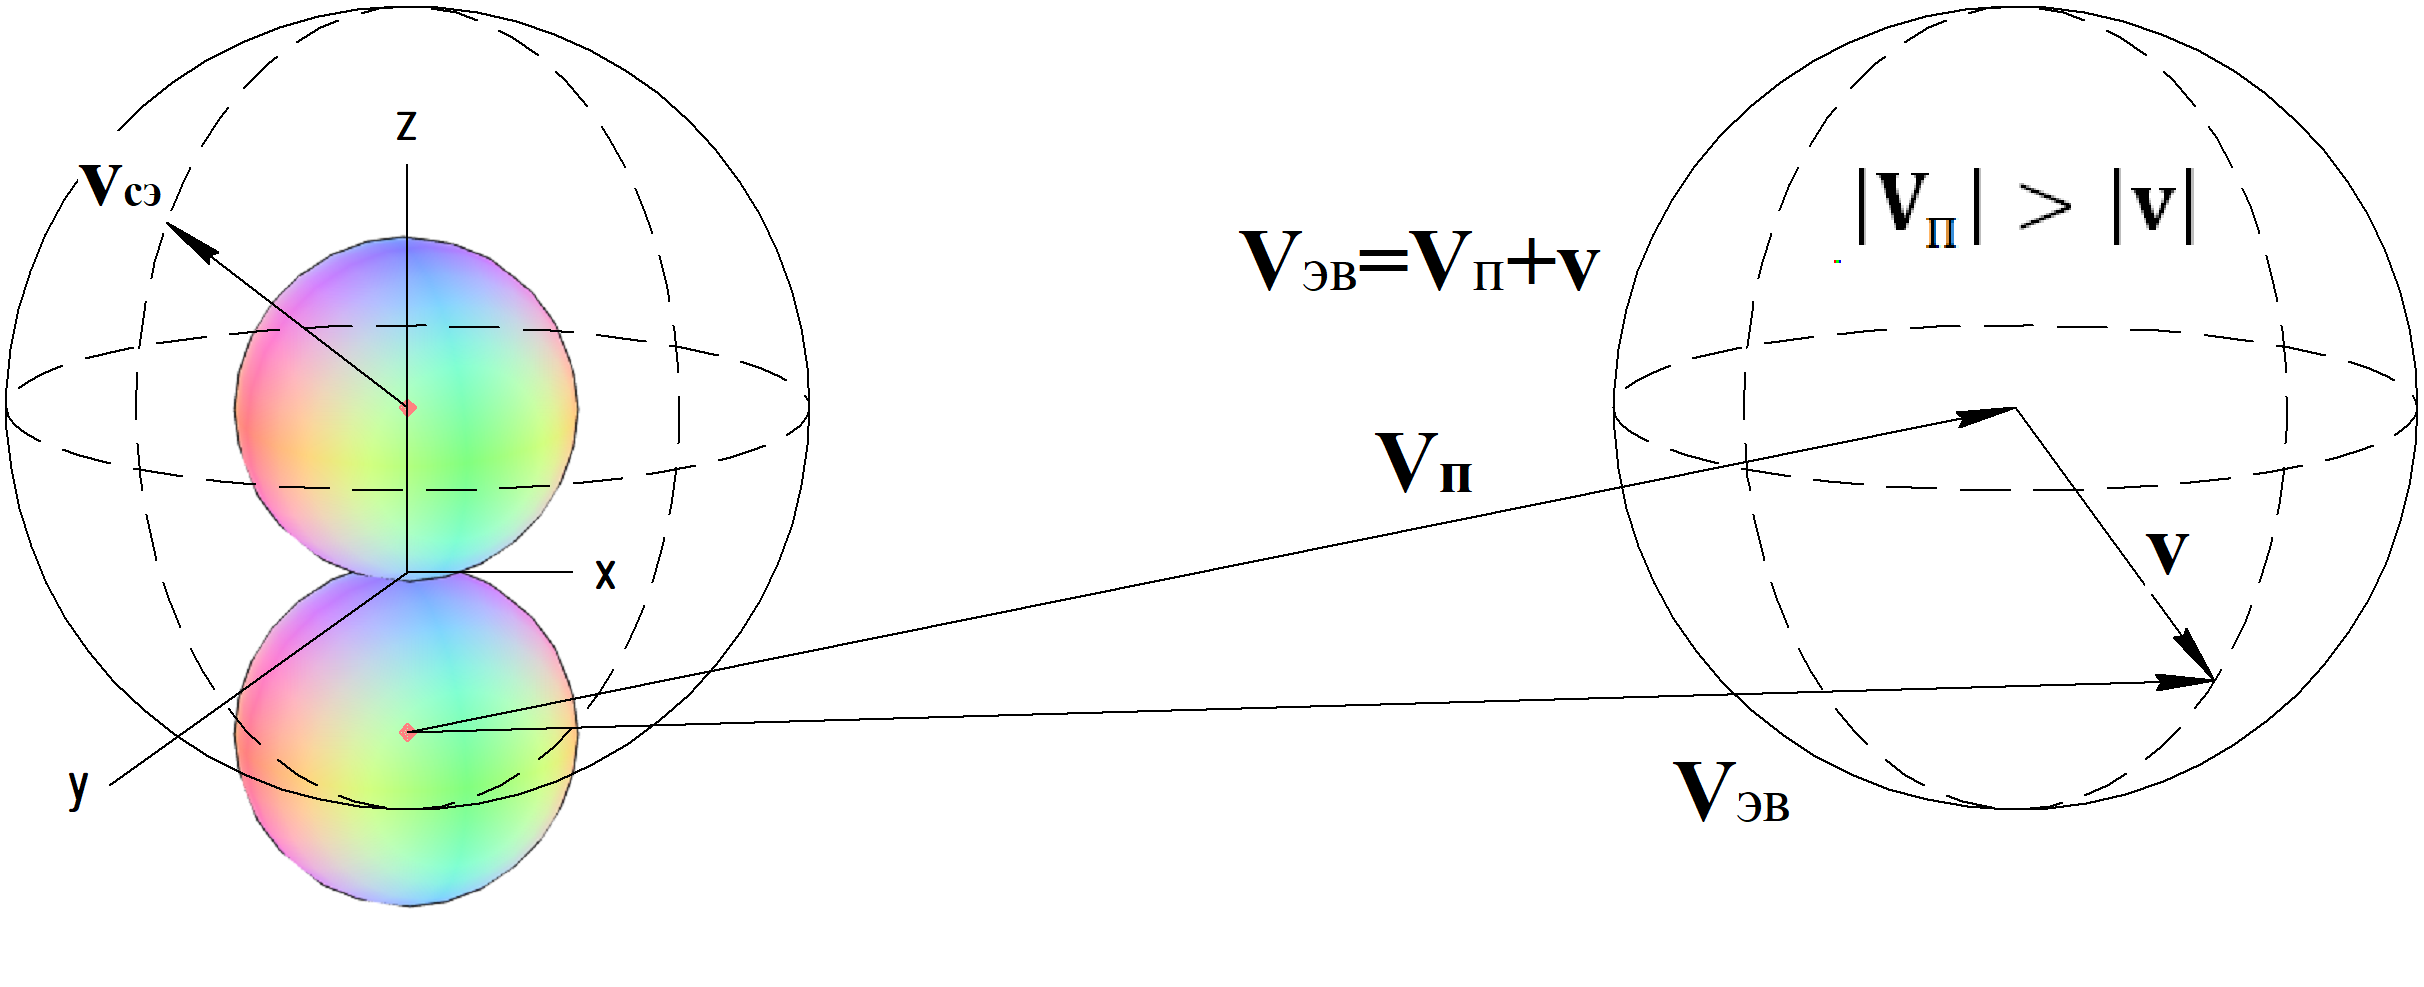
\includegraphics[width=0.55\textwidth]{images/a17.png}
\caption{Схема соударения на границе.}
\label{fig:collision_detail}
\end{figure}

С целью пространственного позиционирования процесса соударения в качестве ориентира используем спиралевидные траектории вихревого движения Амеров, в окрестности которых прецессирует вектор \(\mathbf{v}_{\text{эв}}\), а вектор \(\mathbf{v}_n\) направлен по касательной в каждый момент времени. Как видно из рис. \ref{fig:collision_detail} и следует из условия отсутствия взаимопроникновения частиц через поверхность границы раздела, направления «прилёта» Амеров СЭ к границе ЭВ ограничены величиной телесного угла \(2\pi\), правда, принимая в учёт кривизну поверхности тора, имеющую положительную и отрицательную величины, указанное ограничение имеет соответствующие им отклонения, которые на настоящем этапе в расчёт приниматься не будут. Диаграмма скоростей и направлений движения Амеров ЭВ, приведённая на рис. \ref{fig:cone}, ограничена телесным углом \(\Omega_{\text{пр}}\), предельная величина которого определяется квадратом отношения величины «хаотической» компоненты \(\mathbf{v}\) к величине скорости потока частиц эфира \(\|\mathbf{v}_n\|\).

Какую цель преследует автор, изображая диаграммы скоростей и выясняя особенности в поведении частиц эфира? Обнаружение условий существования обусловленности кинетических параметров частиц СЭ и ЭВ, позволяющих реализовать стационарный протекающий процесс их упругих столкновений, результатом которого будет сохранение целостности вихревых эфирных континуумов.

Продолжая далее рассмотрение рис. \ref{fig:collision_detail}, нужно отметить, что зона точек касания при соударениях Амеров СЭ и ЭВ сосредоточена в области \textbf{сферических сегментов}, прилегающих к этим точкам, так как увеличение возможной зоны контактов приводит к значительному «взаимному проникновению» частиц эфира за условную граничную поверхность ЭВ, что делает процесс столкновений случайным и приводит к нарушению целостности ЭВ, а в случае если \(\|\mathbf{v}_n + \mathbf{v}\| > \|\mathbf{v}_{\text{сэ}}\|\) площадь зоны сосредоточения ударов может сократиться в два раза. Относительно направления скорости потока \(\mathbf{v}_n\) зоной сосредоточения столкновений является «лобовая» часть сферического сегмента Амеров ЭВ и обратная часть сферического сегмента Амеров СЭ. Это предположение о возможном сценарии последовательности событий, соответствие которого истинному предстоит выяснить путём его кинетического анализа с привлечением инвариантов и сделанных ранее выводов, в том числе о равенстве потоков количества движения через граничную условную поверхность раздела ЭВ и СЭ. Равенство масс Амеров, являющихся материальным воплощением движущейся материи, упрощает кинетический анализ процессов соударения на границе раздела, позволяя оперировать векторами скоростей и их абсолютными величинами. При анализе будем использовать факт того, что скорость вихревого движения Амера в теле вихря представляет собой геометрическую сумму скорости направленного вихревого потока и мгновенных значений скорости хаотического движения, непрерывно изменяющихся в процессе соударений Амеров при перемещении в потоке: \(\mathbf{v}_{\text{эв}} = \mathbf{v}_n + \mathbf{v}\). С целью упрощения анализа, ввиду необходимости получения пока качественных суждений о процессе соударений на границе, рассмотрим двумерные варианты возможного развития событий. В процессе сравнительного анализа важно понимать, что будет являться мерой сравнения, и в этом вопросе на первый план выступает свободный эфир с его доминантной ролью главного актора процесса мироустройства в пределах наблюдаемой Вселенной.

\begin{figure}[h]
\centering
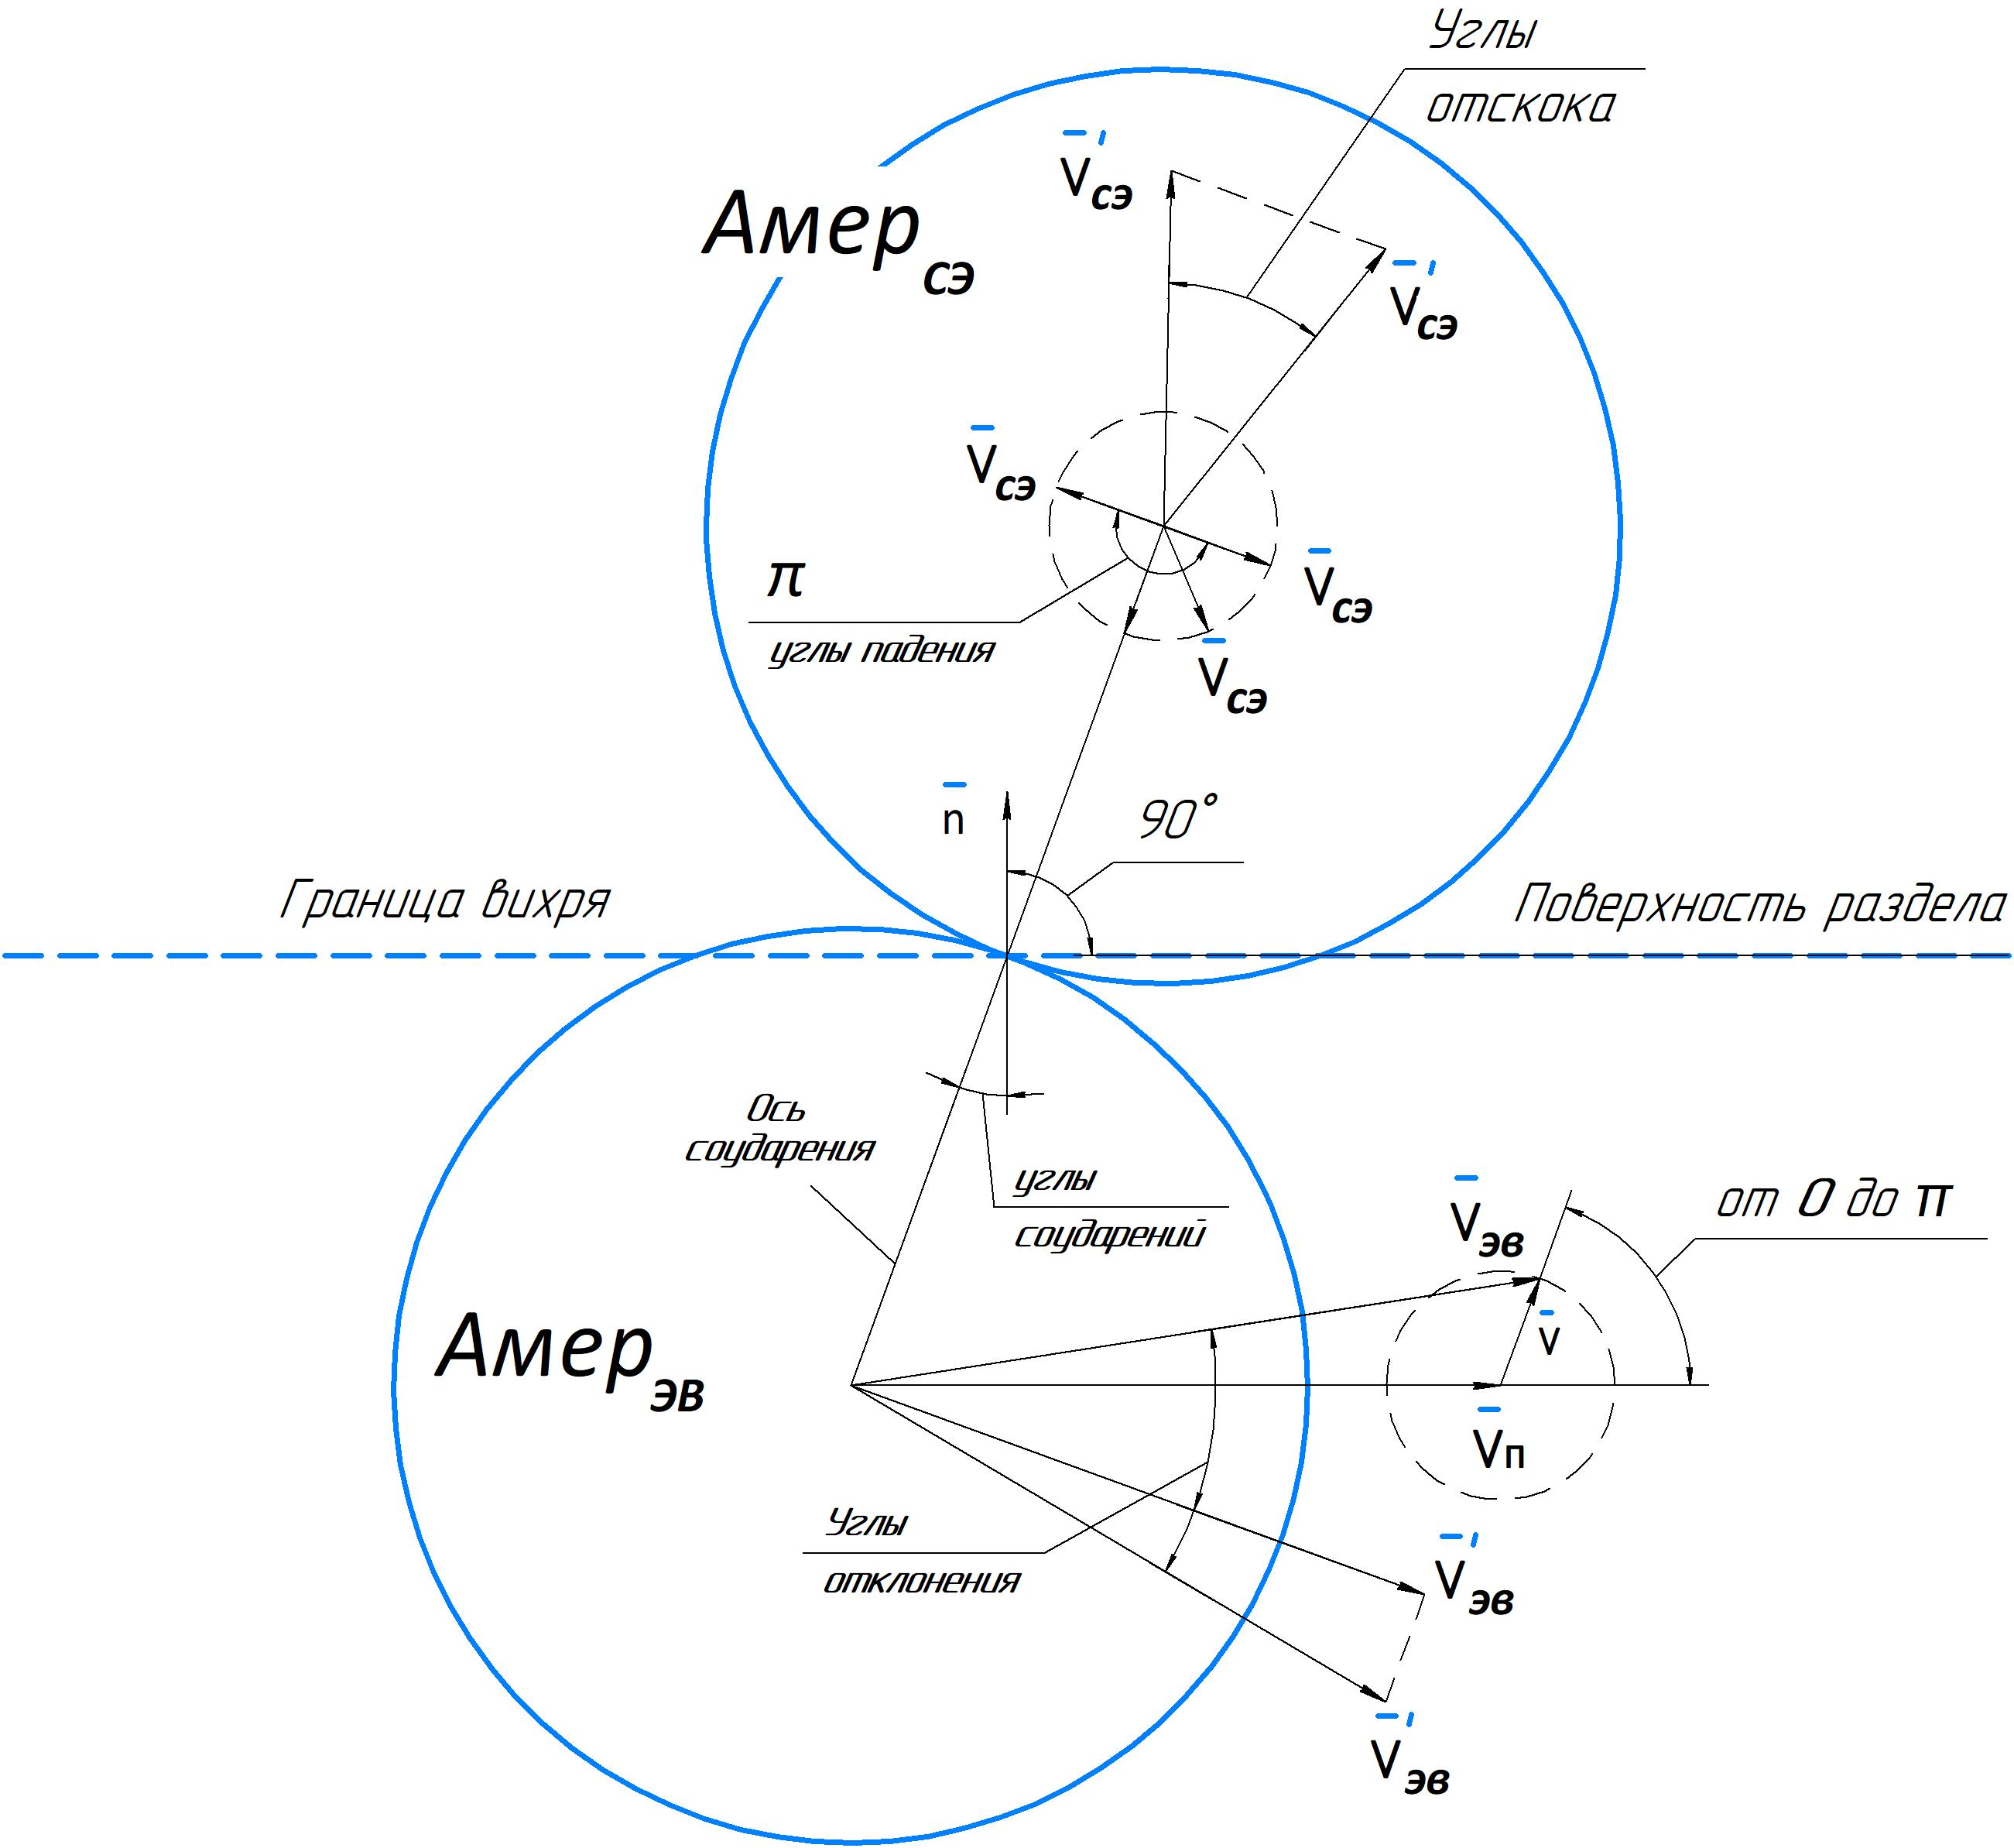
\includegraphics[width=0.55\textwidth]{images/a25.png}
\caption{Эпюра скоростей соударения.}
\label{fig:collision_ab}
\end{figure}

На рис. \ref{fig:collision_ab} (а) изображена схема соударения двух Амеров на условной границе раздела СЭ и ЭВ с использованием методики, позаимствованной автором у Ландау Л.Д. и Лифшица Е.М. (Механика, ТФ, т.1, 1988). Обозначения скоростей были приведены ранее, а знак «\('\)» означает скорости после акта соударения. Центры Амеров соединены линией — \textbf{осью соударения}, проходящей через точку их касания, из которой ортогонально поверхности раздела проведён единичный вектор \(\mathbf{n}\), задающий её ориентацию и направленный в сторону СЭ. Условно радиус окружности Амера СЭ принят равным среднему значению абсолютной скорости хаотического движения Амеров в СЭ \(\|\mathbf{v}_{\text{сэ}}\|\), а вектор скорости потока частиц в ЭВ \(\mathbf{v}_n\) параллелен граничной поверхности раздела СЭ и ЭВ, которая также условно в окрестности точки соударения считается плоской. Схема на рис. \ref{fig:collision_ab} по сути является изображением моментального сечения процесса соударения плоскостью, содержащей вектор \(\mathbf{n}\) и параллельной вектору потока \(\mathbf{v}_n\), поэтому присутствующие на ней углы являются плоскими «образами» своих пространственных, телесных «оригиналов».

Касательно Амеров СЭ можно с уверенностью утверждать, что углы их падения находятся внутри телесного угла \(2\pi\); однако, как видно из рис. \ref{fig:collision_ab}, не каждому углу падения из обозначенного диапазона соответствует событие в виде акта соударения. Если на рис. \ref{fig:collision_ab}(а) положительный результат достигается на любом возможном направлении угла падения в пределах диапазона возможных значений, то на рис. \ref{fig:collision_ab}(б) соударения случаются вдвое реже при той же конфигурации параметров и направлении эфирного потока \(\mathbf{v}_n\), что является прямым следствием изменения значения \textbf{угла соударения} между вектором \(\mathbf{n}\) и \textbf{осью соударения} Амеров. Зависимость возникновения соударений от взаимной ориентации их оси и граничной поверхности даёт основание предполагать существование существенных ограничений величины площади шаровых сегментов поверхности Амеров, в которых сосредоточены точки касания столкновений частиц ЭВ и СЭ.

Следующими вариативными параметрами кинетического анализа являются скорость потока эфирных частиц \(\mathbf{v}_n\) и хаотическая составляющая \(\mathbf{v}\) скорости Амера эфирного вихря \(\mathbf{v}_{\text{эв}}\). Требование \textbf{сплошности} направленного потока частиц ЭВ, движущихся по криволинейным траекториям, предполагает \(\|\mathbf{v}_n\| = \text{const}\), а изменение его направления есть результат обмена компонентами скоростей, коллинеарными \textbf{оси соударения} Амеров на границе СЭ и ЭВ. Под сплошностью подразумевается такая концентрация \(n_{\text{эв}}\) направленно движущихся, соударяющихся частиц эфира, при которой при всех возможных вариантах сочетаний \(\mathbf{v}_n\) и \(\mathbf{v}\) невозможно проникновение Амеров СЭ через граничную поверхность. При этом, что вполне очевидно и логично, речь идёт о всех частицах эфирного потока, а не только сосредоточенных в его приграничном слое.

Согласно диаграммам скоростей, представленным на рис. \ref{fig:collision_ab}, произвольная/хаотичная направленность скорости \(\mathbf{v}\) внутри окружности (а в пространственной реальности — внутри сферы) в пределах обозначенных углов оказывает значительное влияние на длину вектора мгновенной скорости \(\mathbf{v}_{\text{эв}}\) частицы ЭВ, а значит и на величину её «обменной» проекции вдоль \textbf{оси столкновения}, которая, в свою очередь, отвечает за баланс потоков импульса на граничной поверхности ЭВ, о чём подробно было изложено выше. Там же были изложены аргументы в пользу того, что область, отвечающую гармоничному балансу параметров влияния, следует искать при \(\|\mathbf{v}_n\| > \|\mathbf{v}\|\). Из приведённых диаграмм видно, чем больше отношение \(\|\mathbf{v}_n\| / \|\mathbf{v}\|\), тем меньше влияние хаотической составляющей \(\mathbf{v}\) на величину скорости \(\mathbf{v}_{\text{эв}}\), что, в свою очередь, приводит к появлению прогнозируемого результата процесса соударений Амеров на граничной поверхности ЭВ — уменьшению величины \textbf{угла соударений} и появлению \textbf{эффекта отставания} Амеров СЭ от Амеров ЭВ на «догонных» траекториях и в зоне углов боковых столкновений (перпендикулярно плоскости рис. \ref{fig:collision_ab}). Становится возможным существование сценария столкновений частиц эфира на границе ЭВ, при котором они локализуются в ограниченных \textbf{активных зонах} в виде половинок шаровых сегментов у сталкивающихся на граничной поверхности пар Амеров. Ограничение области локализации столкновений в окрестности точек контакта, обусловленное пространственной геометрией частиц эфира, в окрестности граничной поверхности ЭВ автор назвал \textbf{скольжением}. Скольжение — это искомое сочетание кинетических параметров, из их (сочетаний) бесконечного числа, при котором становится возможным автовозобновляемый процесс существования долго «живущих» пространственно локализованных континуумов вихревой эфирной материи.

Следование избранным модельным предположениям, инвариантам и физической логике, а также материалистическим представлениям о природе материи и бытия позволили установить ряд важных, необходимых и достаточных условий существования вихревых эфирных структур, служащих прообразами элементарных частиц вещественной материи. Особый физический сценарий соударений частиц на границе ЭВ и СЭ, реализуемый в виде \textbf{скольжения}, указывает на малую, составляющую доли \(d_a\), «\textbf{толщину}» области сосредоточения соударений у граничной поверхности. Таким образом, геометрическим условием осуществления ЭВ является локализация точек касания сталкивающихся Амеров СЭ и ЭВ на половине площади шарового сегмента в окрестности точки пересечения \textbf{оси соударения} и вектора граничной поверхности вихря \(\mathbf{n}\).

\begin{figure}[h]
\centering

\includegraphics[width=0.25\textwidth]{images/a13.png}
\caption{Локализация области соударений.}
\label{fig:localization}
\end{figure}

\begin{figure}[h]
\centering
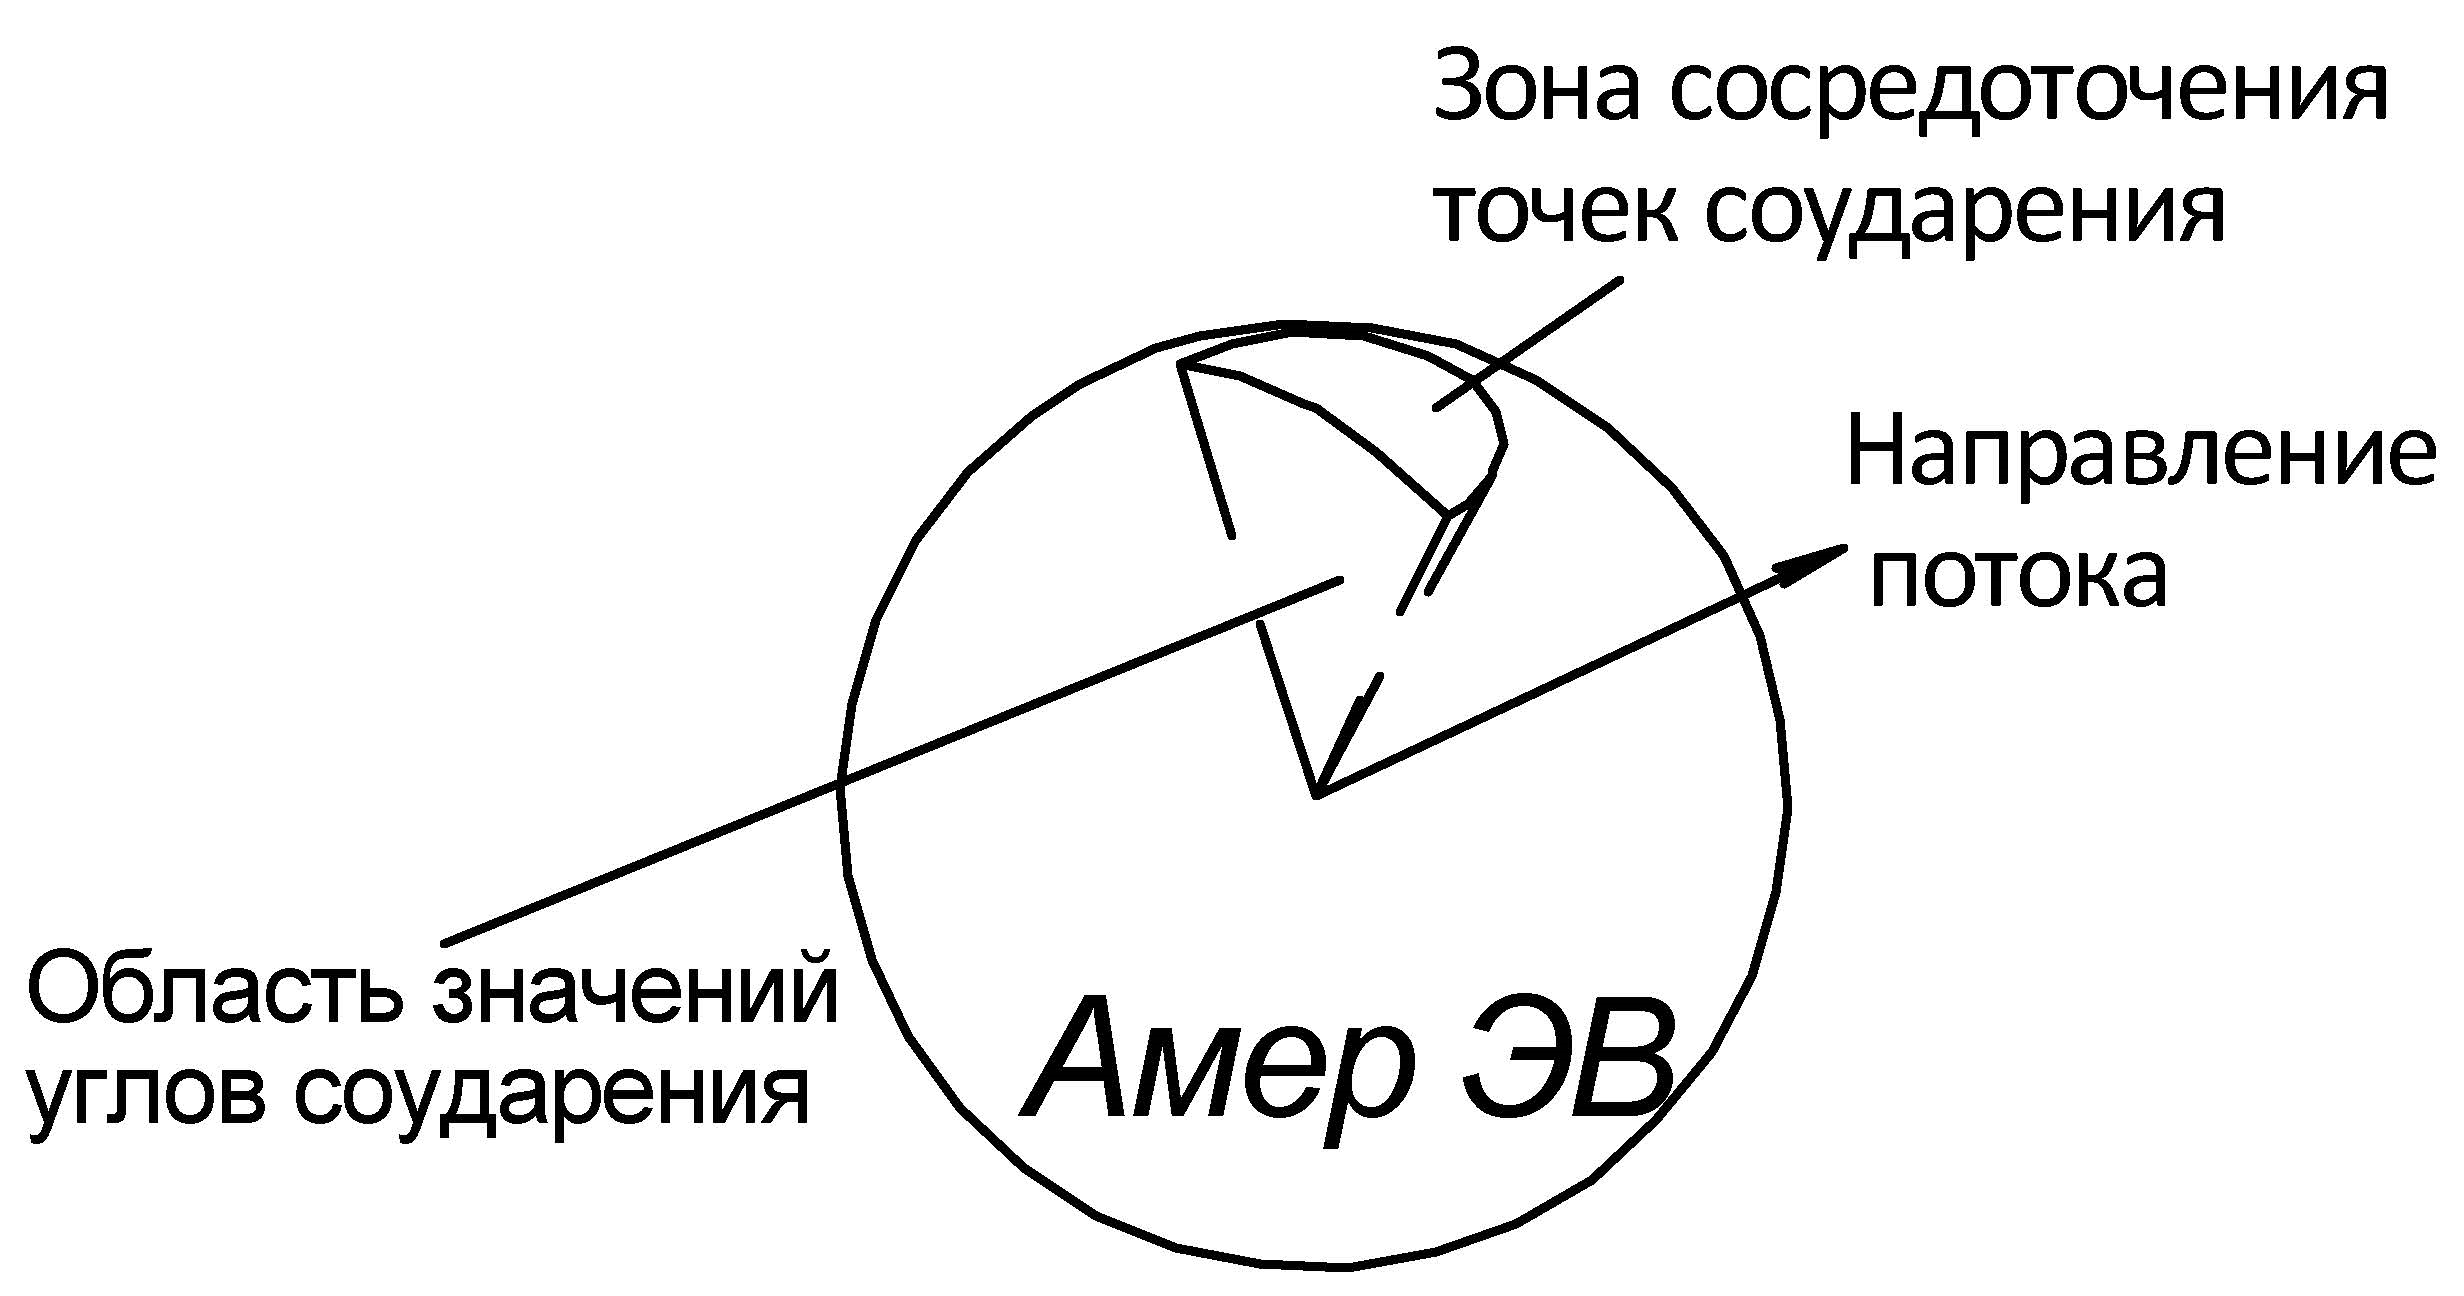
\includegraphics[width=0.55\textwidth]{images/a14.png}
\caption{Схема скольжения.}
\label{fig:sliding}
\end{figure}

Это условие также может быть сформулировано в виде детерминантного ограничения на совокупность возможных значений \textbf{вероятных углов соударений}, составляющих телесный угол, эквивалентный половине площади шарового сегмента поверхности Амера — месте сосредоточения точек касания соударений, которое определяется из условия баланса количества движения через граничную поверхность и взаимообусловленности кинетических и геометрических параметров среды СЭ и ЭВ.

Равенство потоков импульса через границу эфирного вихря и отсутствие взаимопроникновения частиц не отрицает простой и очевидный факт абсолютного равенства числа участвующих в соударениях на граничной поверхности Амеров СЭ и ЭВ, из чего при \(\|\mathbf{v}_n + \mathbf{v}\| \gg \|\mathbf{v}_{\text{сэ}}\|\) следует, что за единицу времени на единице площади граничной поверхности выполнение такого равенства возможно, если \(n_{\text{сэ}} > n_{\text{эв}}\). Аргументом в пользу того, что свободный эфир плотнее эфирного вихря, служат слова Николы Теслы, приведённые в интервью корреспонденту Нью-Йоркской газеты, об образном представлении эфирных вихрей в виде пузырьков воздуха в воде, которая является аналогом среды свободного эфира или физического вакуума. В связи с этим представляет интерес смысловое содержание параметра эфирной среды в виде произведения концентрации частиц эфира и среднего значения модуля их скорости применительно к СЭ, ЭВ и процессу столкновений Амеров на их границе. В классической физике указанный параметр носит название \textbf{плотности потока} (\(j\)) некоторой «субстанции», распределение которой описывается стационарной векторной функцией, определённой в каждой точке пространства, или стационарным векторным полем и, в общем случае, является векторной величиной. Применительно к эфиру, а именно к СЭ, можно с уверенностью утверждать, что в силу пространственной изотропности его свойств и стационарности протекающих процессов величина плотности потока \(j\) составляющих его Амеров имеет нулевую величину во всех направлениях, в том числе через граничную поверхность ЭВ. Это утверждение уже приводилось ранее по тексту в виде условия об отсутствии взаимопроникновения Амеров через граничную поверхность ЭВ, что является ещё одним подтверждением в пользу избранной методики анализа. При этом плотность потока импульса в СЭ имеет определённое, не равное нулю значение, одинаковое во всех направлениях в пределах телесного угла \(4\pi\). В отношении ЭВ ситуация диаметрально противоположная в силу направленности движения составляющих его Амеров. Если высказанное автором ранее предположение \(\mathbf{v}_{\text{эв}} = \mathbf{v}_n + \mathbf{v}\) является верным, то логичным будет утверждение о том, что \textbf{плотность потока} частиц ЭВ аналогично представляет собой векторную сумму «направленной» и «хаотической» компонент, а именно \(j_{\text{эв}} = j_n + j\). Согласно определению, потоком какой-либо субстанции через участок поверхности называется скалярное произведение вектора плотности потока этой субстанции и вектора, величина и направление которого определяются вектором пространственной ориентации выбранного участка поверхности \(\mathbf{n}\) и его площадью. Таким образом, поток частиц через участок поверхности ЭВ, согласно свойству дистрибутивности скалярного произведения, представляет собой сумму двух потоков в соответствии с компонентами вектора плотности потока частиц \(j_n\) и \(j\). Принимая во внимание параллельность вектора \(\mathbf{v}_n\) и граничной поверхности, а значит ортогональность векторов \(j_n\) и \(\mathbf{n}\), а также отсутствие взаимопроникновения частиц между СЭ и ЭВ, можно сделать вывод, что при соблюдении условий \textbf{скольжения} \(\|\mathbf{v}_n\| \gg \|\mathbf{v}\|, \|\mathbf{v}_{\text{сэ}}\|\) поток частиц из ЭВ через граничную поверхность отсутствует, что, в свою очередь, является необходимым условием существования вихря. Касательно потока Амеров в теле ЭВ следует отметить, что, несмотря на спиральный вид траекторий частиц, это направленное движение и для него справедливо уравнение \(j_n = n_{\text{эв}} \mathbf{v}_n\), так как поворот вектора скорости \(\mathbf{v}_{\text{эв}}\) происходит по факту как результат «обмена» скоростями при столкновениях с Амерами СЭ, что в совокупности с одинаковой «хаотической» сущностью \(\mathbf{v}_{\text{сэ}}\) и \(\mathbf{v}\) позволяет замкнутому потоку частиц в ЭВ существовать в течение неограниченно долгого времени.

Особый «скользящий» сценарий взаимодействия ЭВ и СЭ на граничной поверхности даёт основания предполагать невозможность уничтожения замкнутых вихревых потоков частиц эфира и, как следствие, возможность их дробления с последующим образованием сложных, в том числе ортогонально ориентированных, взаимно охватывающих (по типу цепных звеньев) пространственных вихревых конструктивов, а также слияния при выполнении соответствующих необходимых этому процессу условий. Вихревые потоки взаимно не уничтожаются; более того, вихри разной направленности прекрасно могут сосуществовать в составе вещественных структур, в том числе элементарных частиц.

Анализируя ранее условия реализации сценария скольжения на граничной поверхности ЭВ, автор сделал предположение, что \(n_{\text{сэ}} > n_{\text{эв}}\), означающее большую плотность СЭ по отношению к ЭВ. Однако дальнейшее обоснование этого тезиса в части сохранения направленности движения потока частиц эфира приводит к необходимости существования детерминантного ограничения на среднее значение длины свободного пробега частицы в СЭ. Если это значение таково, что Амеры имеют возможность свободного движения между соседними частицами, то возникают условия для «вылета» имеющих значительно большую скорость Амеров из потока ЭВ за пределы его граничной поверхности, что, в свою очередь, приводит к нарушению условий существования сценария \textbf{скольжения}. Таким образом, если максимальное значение длины свободного пробега частицы в СЭ будет меньше диаметра Амера (\((\lambda_{\text{сэ}})_{\max} < d_a\)), то возникает «запрет на свободный проход» между соседними частицами, из чего следует, что величина концентрации частиц эфира \(n_{\text{сэ}}\) в нём должна быть достаточной для физической реализации такого запрета. Ограничение длины свободного пробега частиц эфира в СЭ \(0 < \lambda_{\text{сэ}} < d_a\) естественным образом поднимает вопрос: «С чем это можно сравнить? Или какую из известных материальных систем можно выбрать в качестве аналога?» Ранее по тексту автор делал ссылку на «газообразную» и «сыпучую» структуры среды эфира, оценивая возможности моделирования устойчивых локальных эфирокинетических континуумов на основе предлагаемых другими авторами оценок \(\lambda_{\text{сэ}}/d_a\), предполагая, конечно, при этом в качестве модельной основы «газоподобный» эфир. Среда эфира представлена абсолютно твёрдыми, плотно упакованными, но подвижными Амерами, и в совокупности свойств аналогична поведению «псевдоожиженных» твёрдых смесей, и в силу этого автор взял на себя ответственность наделить эфир свойствами «\textbf{псевдожидкости}».

Надо отметить, что в системе отсчёта, движущейся параллельно граничной поверхности ЭВ со скоростью \(\mathbf{v}_n\) (рис. \ref{fig:collision_ab}), Амеры пребывают в хаотическом движении. Так как вектор скорости потока \(\mathbf{v}_n\) и вектор граничной поверхности \(\mathbf{n}\) ортогональны, среднее значение проекции этой скорости на ось соударений частиц эфира равно нулю, что исключает вклад «направленной» части движения в процесс обмена импульсами при столкновениях Амеров на граничной поверхности раздела СЭ и ЭВ.
